%Text Check!
\section{Method}

\subsection{Wave Channel}

The extension of the water tank was necessary since the original channel was too short for the new wavemaker. Also, additional devices such as a coastal model and a wave absorber were built. It will be discussed in this section.

\subsubsection{Wave Channel Extension}%Check!

The wave channel was extended to $6,000\mathrm{~mm}$ to get extra space for the coastal model, wavemaker, and a domain for wave generation. A new module was built similarly, with the framework of the aluminum profile 3030 series (cross-sectional area $30\mathrm{~mm} \times 30\mathrm{~mm}$) and the inner wall of an acrylic plate ($5\mathrm{~mm}$ thickness), with its dimension $2,000\mathrm{~mㅡ}$ $\times$ $300\mathrm{~mm}$ $\times$ $400\mathrm{~mm}$. It was inserted in the middle of the other two.

The wave channel needed sealing between the modules to prevent water leakage. Silicone pads were cut into U-shapes so that they fit right into the section where the aluminum profile meets. Also, acrylic rods were attached to each side of the modules and long bolts passed through them, tightening the link and pressing silicone pads.


\begin{figure}[H]
    \begin{center}
        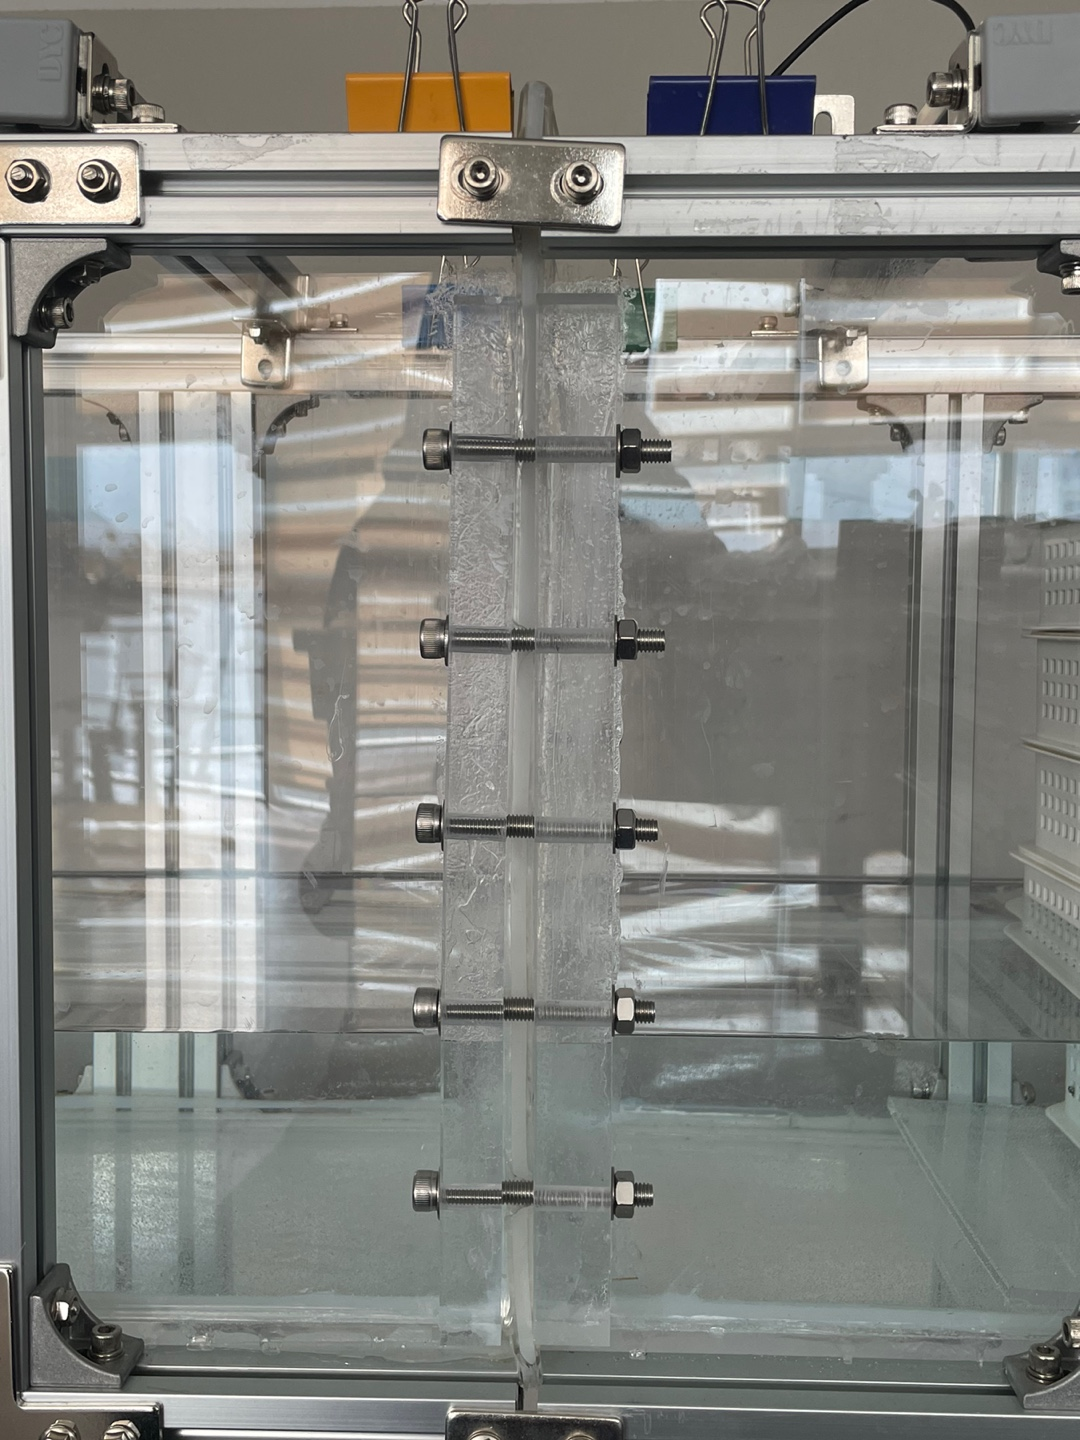
\includegraphics[height=5cm]{images/Connection(Side).jpg}
        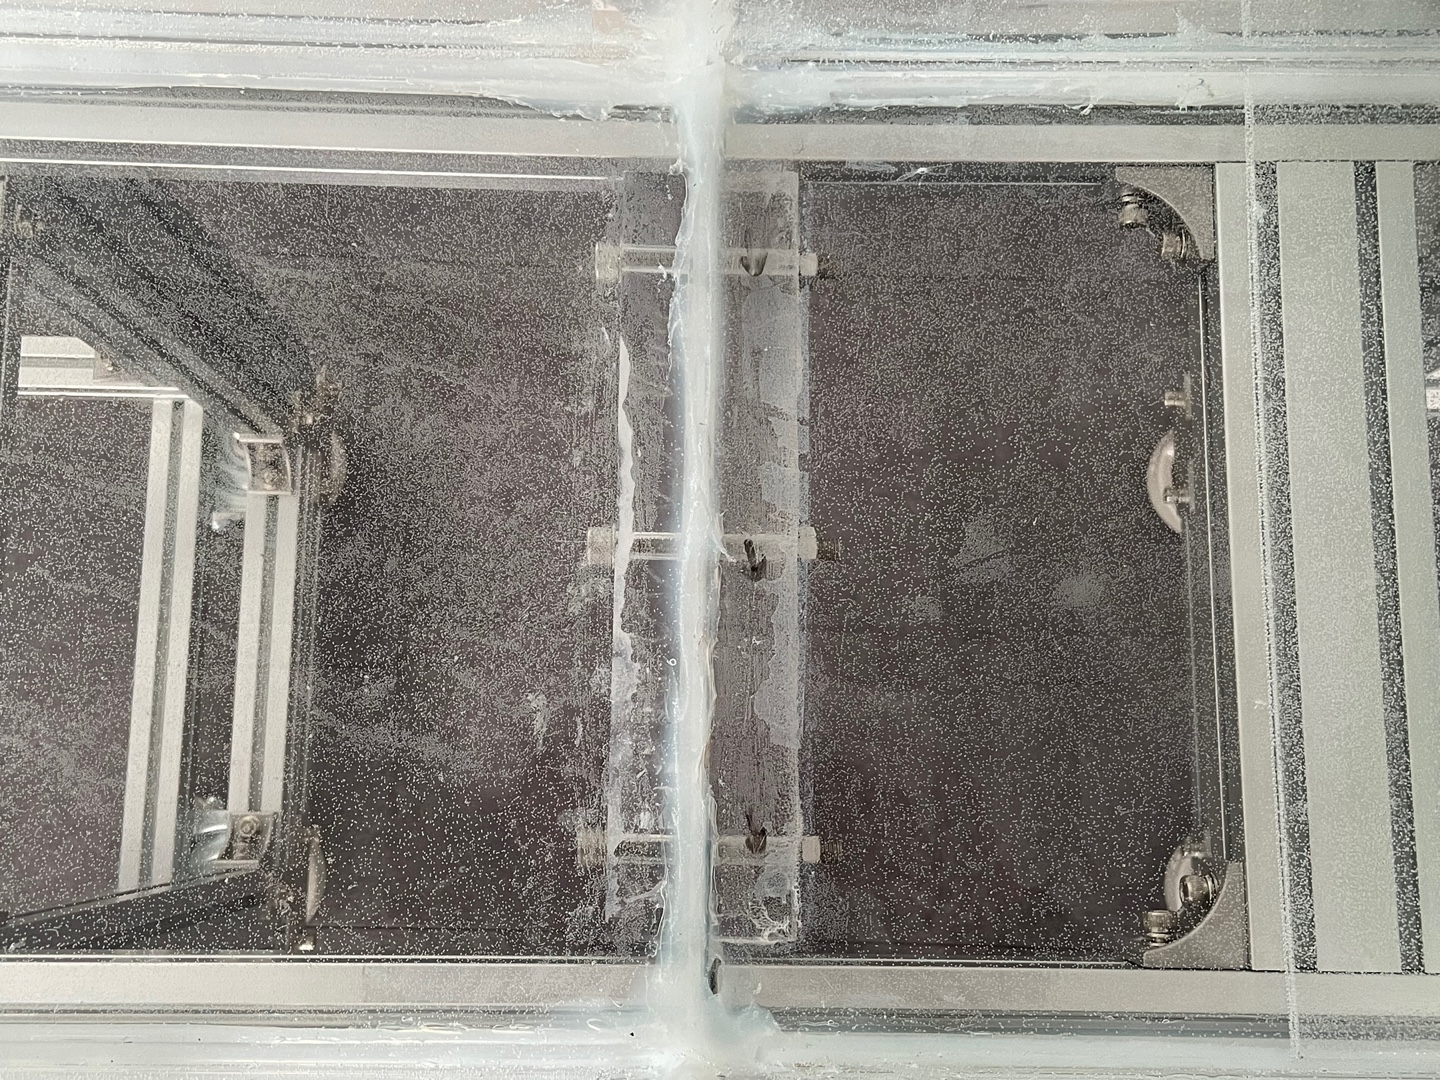
\includegraphics[height=5cm]{images/Connection(Silicone).jpg}
    \end{center}
        \begin{tikzpicture} [remember picture, overlay]
            \node at (2.1, 0.6) {\scriptsize{(a)}};
            \node at (6.0, 0.6) {\scriptsize{(b)}};
        \end{tikzpicture}
        \caption{Connection of the modules - (a) side (b) bottom}
        \label{connection} 
\end{figure}

Lastly, smaller gaps were sealed with a silicone gun. Smaller gaps were spotted from the water leakage when water was poured. After a few trial-and-error, the wave tank was sealed completely (Figure \ref{wave channel}). Also, the entire tank must be straight and flat overall. All three modules needed to be aligned straight. There are four wheels at the bottom of each module with a screw so that the height can be adjusted by tightening it.

\begin{figure}[H]
    \centering
    %\captionsetup{justification=centering}
    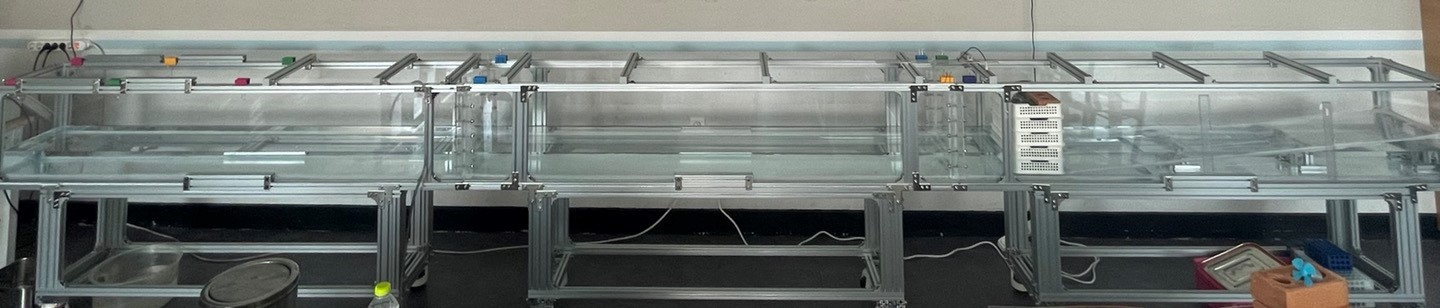
\includegraphics[width=\textwidth]{images/Wave_Tank(without_Generator).jpg}
    \caption{Wave channel}
    \label{wave channel}
\end{figure}

\subsubsection{Wave Absorber}%Check!

As the plate moves back and forth, waves that do not go in the direction of the coastal model must be extinguished to reduce systematic error. These waves could interfere in a region behind the wavemaker, exerting force on the plate. There is an existing wave absorber, a rectangular parallelepiped with holes in a three-dimensional grid printed with a 3D printer. The holes were not completely perforated but filled with wires and they effectively extinguish the wave.

According to previous studies, the wave absorber that can be made and installed to the wave channel in the lab is a rectangular parallelepiped brick of a porous structure like the previous one. Based on this idea, the prototype was made with a stainless steel box, with holes drilled through. But it was too difficult to handle and the box was void: Not proper to play the role. Thus, the baskets with holes were used, filled with scrubbers. The baskets fit in the wave channel, stacked into five floors. There is a way to test the ability of a wave absorber, but generating a proper sinusoidal wave is before it.

\begin{figure}[H]
    \begin{center}
        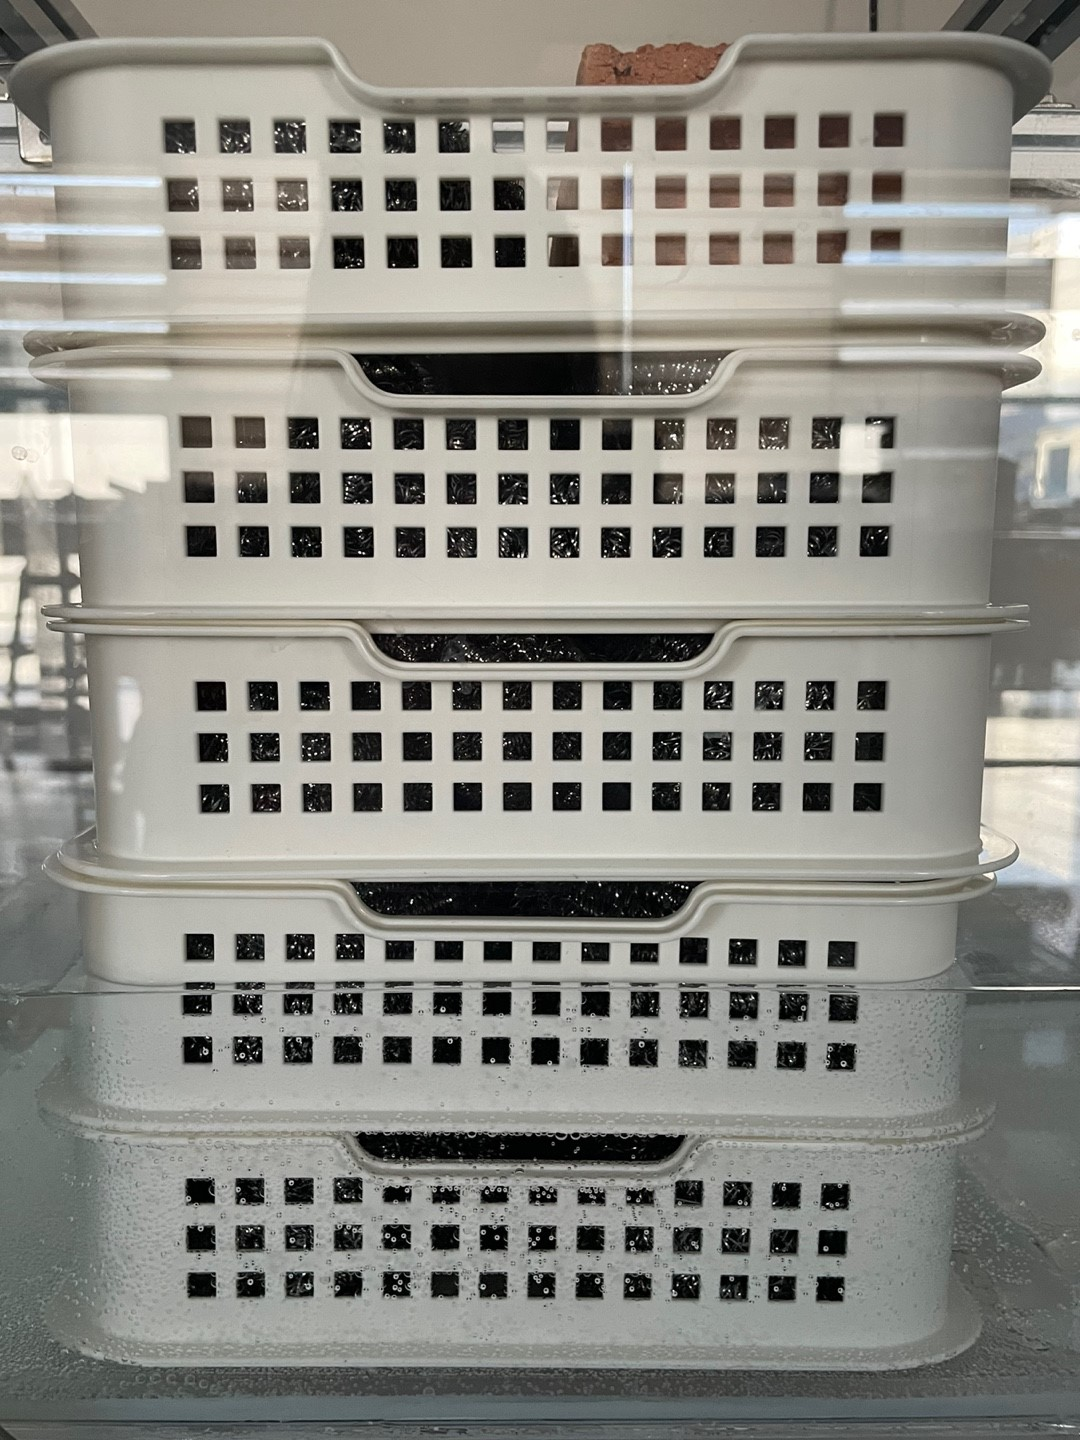
\includegraphics[width=5cm]{images/Wave_Absorber(Side).jpg}
        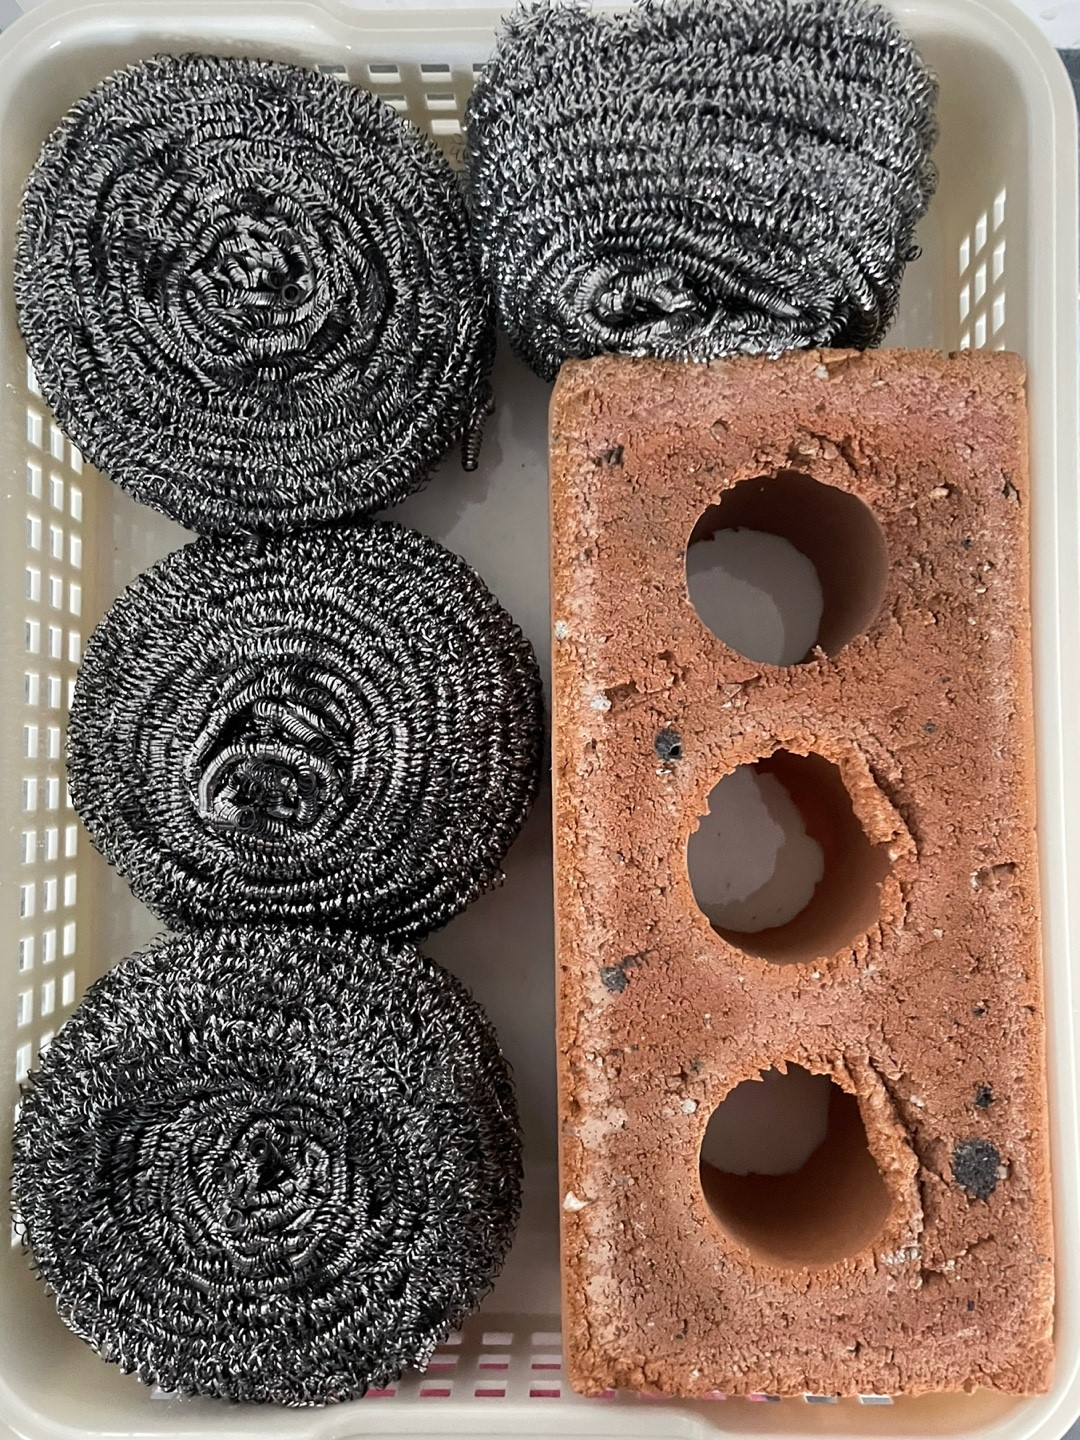
\includegraphics[width=5cm]{images/Wave_Absorber(Top).jpg}
    \end{center}
        \begin{tikzpicture} [remember picture, overlay]
            \node at (2.3, 0.6) {\scriptsize{(a)}};
            \node at (7.5, 0.6) {\scriptsize{(b)}};
        \end{tikzpicture}
        \caption{Wave absorber - (a) side (b) top}
        \label{Experimnet_System} 
\end{figure}

\subsubsection{Coastal Model}%Check!

A ramp was made as the coastal model. It would depend on the experiment, but the actual underwater terrain should have a slope from the seabed to the coast. Extra spaces could be provided at the end of the coast, allowing structures to be installed on flat land. Only the ramp was installed with the slope of $1/10$, considering that $1/20$ or $1/10$ is appropriate. Regarding that tank is $6,000\mathrm{mm}$ long and $400\mathrm{mm}$ high, the dimension was set as the length of $2,000\mathrm{m}$ and the height of $200\mathrm{mm}$. Bur for conducting the experiment verifying the generated wave, it needs to be detached.

An acrylic plate with a thickness of $5\mathrm{mm}$ was supported below with pedestals in three steps, made of aluminum profile bars. These pedestals were also detachable (Figure \ref{Coastal_Model(Ramp)}).

\begin{figure}[H]
    \centering
    %\captionsetup{justification=centering}
    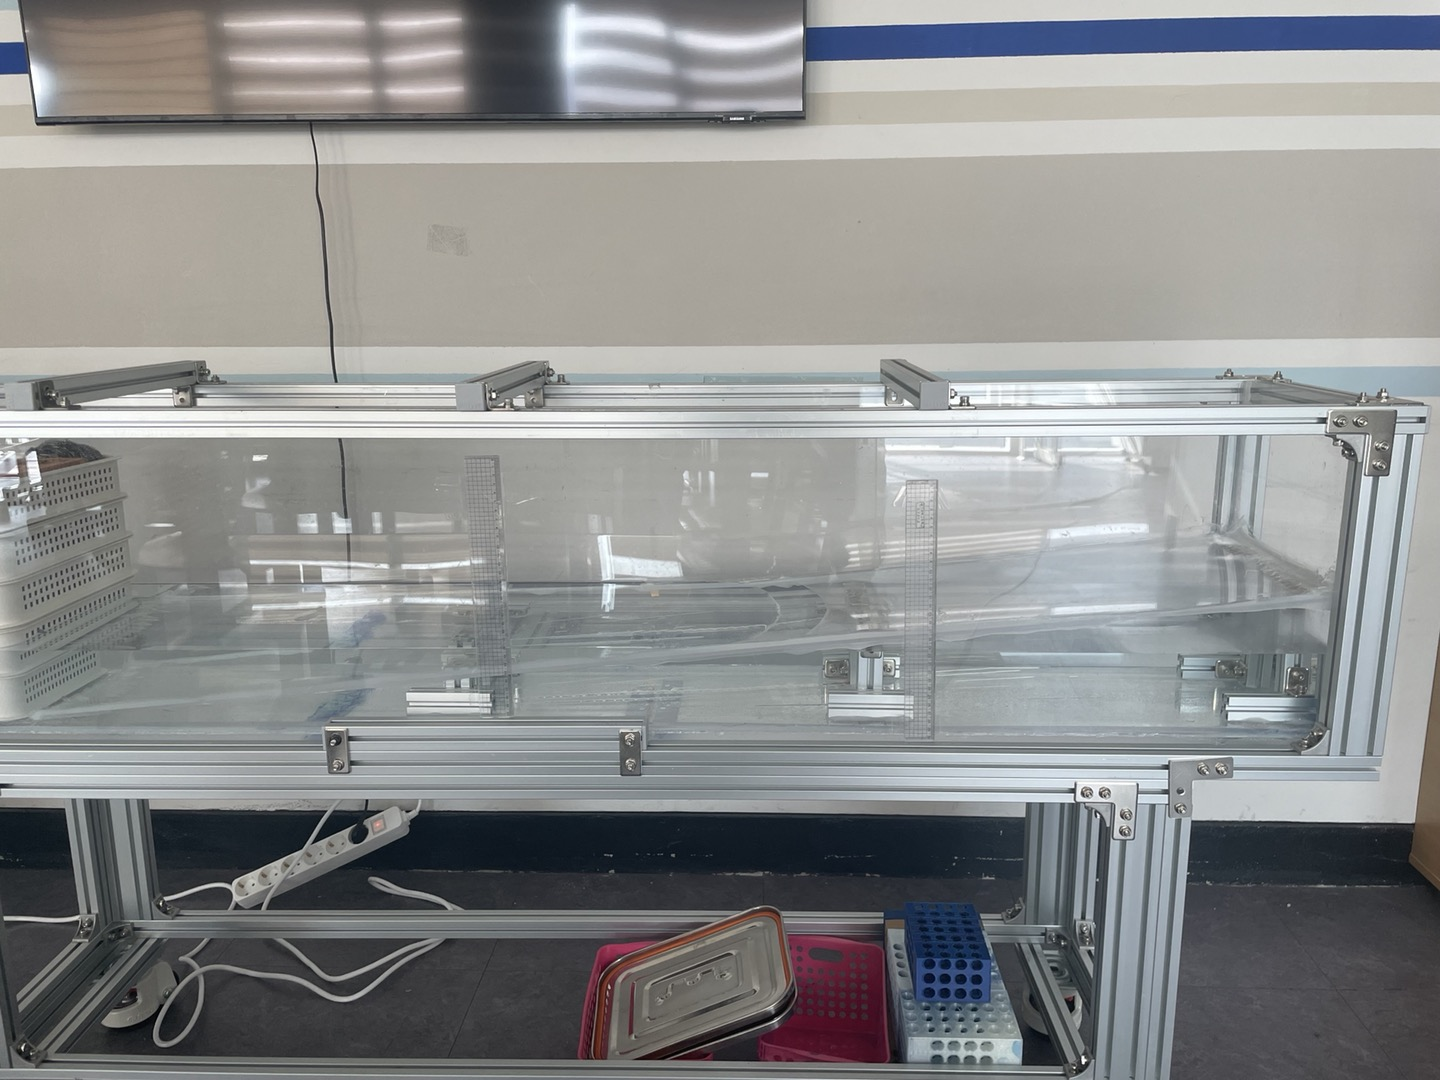
\includegraphics[width=11cm]{images/Coastal_Model(Ramp).jpg}
    \caption{Coastal Model - Ramp}
    \label{Coastal_Model(Ramp)}
\end{figure}

\subsection{Wavemaker}%Check!

The wavemaker consists of a driving unit and a control unit. The driving unit is a mechanical part of the wavemaker that moves the motor, and it is composed of a linear actuator and several structural components. The control unit is a circuit consisting of a motor driver, a Teensy3.2, a transformer, and other circuit diodes and it executes the code.

\begin{figure}[H]
    \centering
    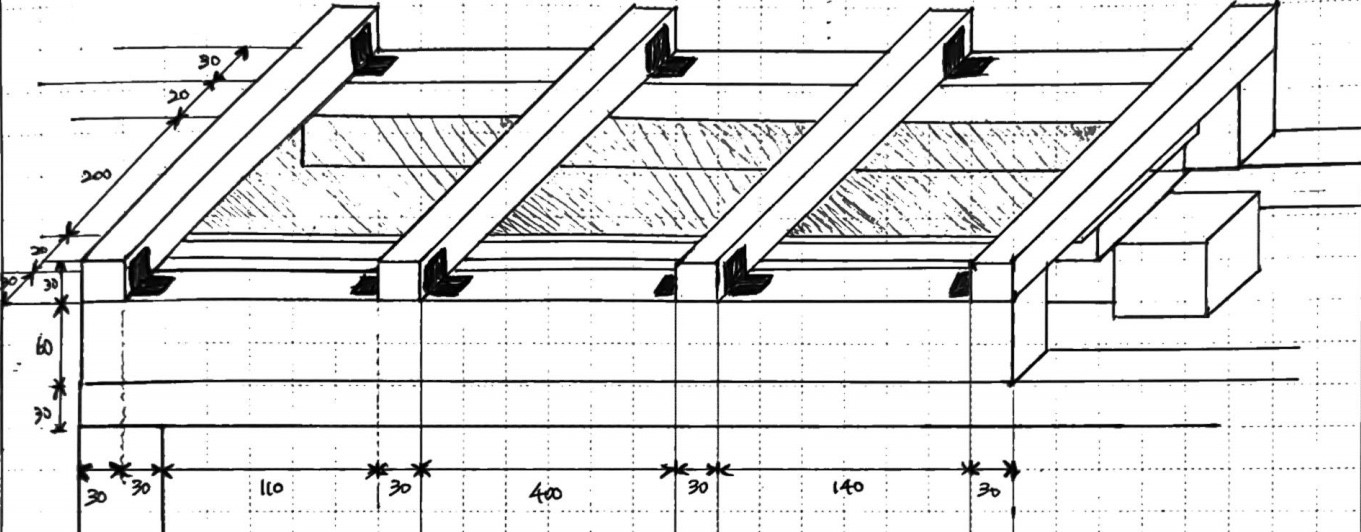
\includegraphics[width=12cm]{images/Wave_Maker(Design_not_drawn_to_scale).jpg}
    
    \caption{The design of the wave channel (Not drawn to scale)}
    \label{Wave_Tank(Design)}
\end{figure}

\subsubsection{Driving Unit}

A main component of the driving unit is a linear actuator, which converts the rotating motion of the motor to translating motion of an object through the screw thread (Figure \ref{linear actuator} The product is the FSK80 series from FUYU, Chengdu. Here is the basic information about the linear actuator.

\begin{table}[H]
    \centering
    \captionsetup{justification=centering}
    \begin{tabular}{l|l}
        \hline
        guide width $(\mathrm{mm})$                       & 80                                     \\
        repeat position accuracy $(\mathrm{mm})$          & +-0.02                                 \\
        motor                                  & stepper 60102                          \\
        rail model                             & dual rail W12 $\times$ H8              \\
        ball screw model                       & 16                                     \\
        \textbf{stroke $(\mathrm{mm})$}                  & \textbf{50 - 1000}                                    \\
        pitch                                  & 10                                     \\
        \textbf{horizontal full payload speed $(\mathrm{mm/s})$}   & \textbf{230}                                    \\
        vertical full payload speed $\mathrm{(mm/s)}$     & 60                                     \\
        side mounting payload speed $\mathrm{(mm/s)}$     & 210                                    \\
        \textbf{rated horizontal payload $\mathrm{(kg)}$}          & \textbf{40}                                     \\
        rated vertical payload $(kg)$            & 20                                     \\
        rated side mounting payload $(kg)$       & 15                                     \\
        noisy without payload $(db)$             & 79                                     \\
        rated payload noisy $(db)$               & 70                                     \\
        \textbf{acceleration $(mm/s^{2})$} & \textbf{500}                                    \\ \hline
    \end{tabular}%
    \caption{Specification of linear actuator - \textit{FSK80} Series}
    \label{specifiacion of linear actuator}
\end{table}

An $80\mathrm{~cm}$ long linear actuator was used. It is attached to an aluminum board and frameworks (Figure \ref{Wave_Tank(Design)}). The framework consists of an aluminum profile 3030 series. The linear actuator can bear up to $40\mathrm{~kg}$ horizontally, and its maximum speed is $230\mathrm{mm/s}$ with a full payload. The acceleration of the object is $500\mathrm{mm/s^{2}}$.

Limit switches were used to indicate the end of the actuator and the moving range of the motor. It's a sensor that sends out different voltage signals when metal is detected on one side of it (Figure \ref{limit switch}). 2 pieces were used, one at each end of the rail. As the object (the one moving through the rail) passes the switch, metal is detected and the location - angular displacement - is checked to limit the range of the motion.

\begin{figure}[H]
    \begin{center}
        \scalebox{-1}[1]{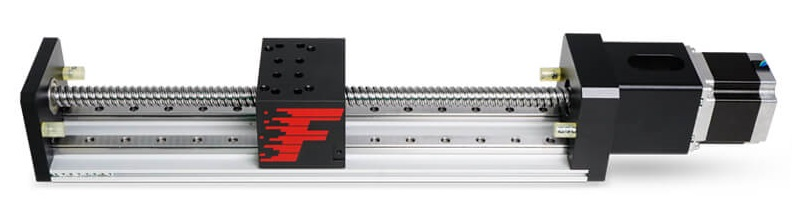
\includegraphics[width = 12cm]{images/Linear_Actuator.jpg}}
        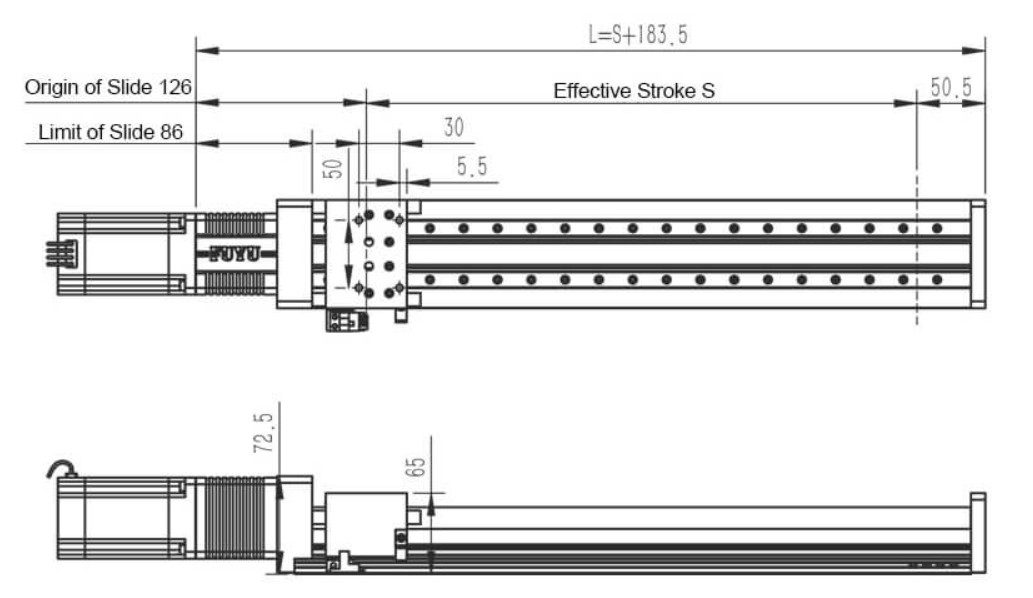
\includegraphics[width = 12cm]{images/Linear_Actuator(Design).jpg}
    \end{center}
        \begin{tikzpicture} [remember picture, overlay]
        \node at (2.0, 11.0) {(a)};
        \node at (2.0, 7.6) {(b)}; %1.1
        \end{tikzpicture}	
        \caption{Linear actuator - (a) \textit{FSK80} series (b) Design}
        \label{linear actuator}
\end{figure}

\begin{figure}[H]
    \centering
    \captionsetup{justification=centering}
    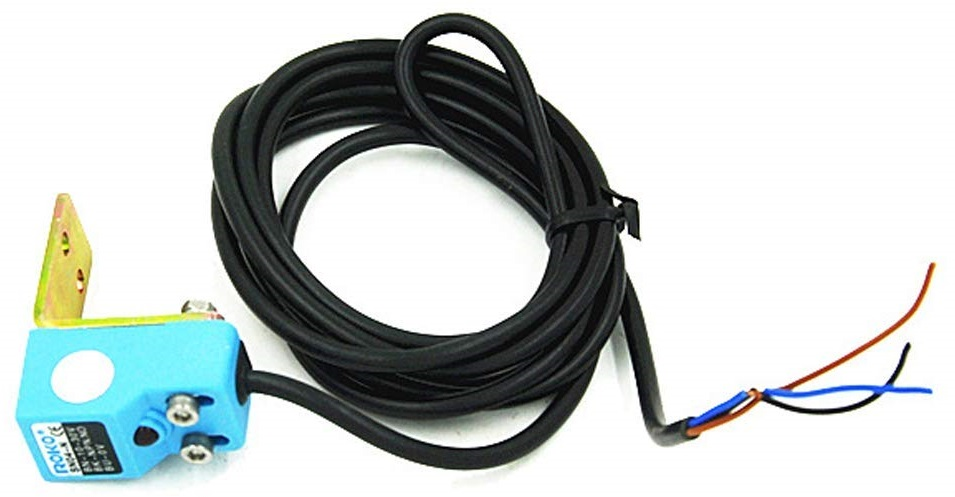
\includegraphics[width = 6cm]{images/Limit_Switch.jpg}
    \caption{Limit Switch}
    \label{limit switch}
\end{figure}

\subsubsection{Control Unit}

The control unit consists of Teensy 3.2, DRV8825, Microstep Driver (ST-M5045), and $24\mathrm{~V}$ SMPS. Teensy 3.2 is a main CPU board and executes the inserted code (Figure \ref{Teensy3.2}). For further information, refer to www.pjrc.com/teensy.

\begin{figure}[H]
    \centering
    \captionsetup{justification=centering}
    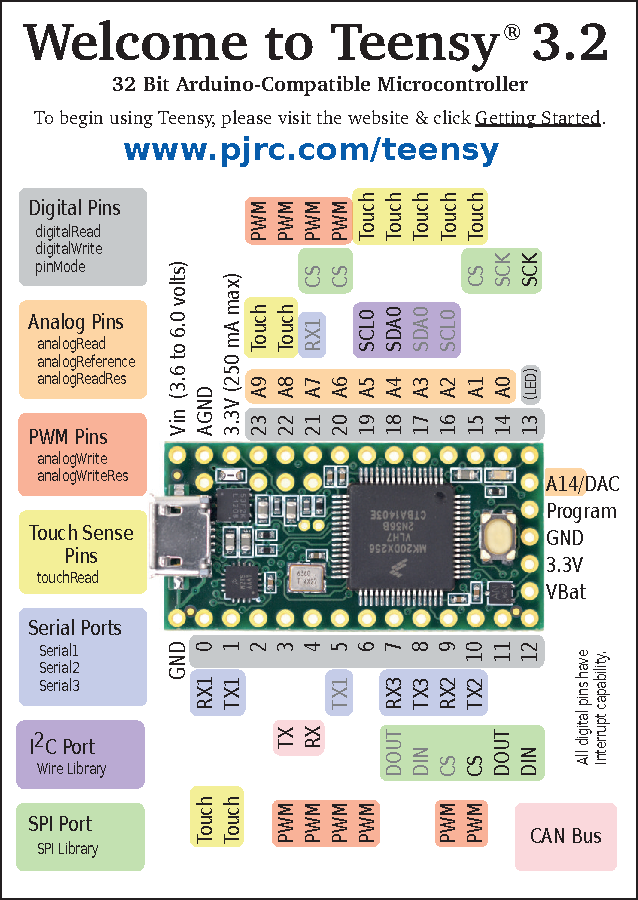
\includegraphics[width=6cm]{images/Teensy3.2 - 1.pdf}
    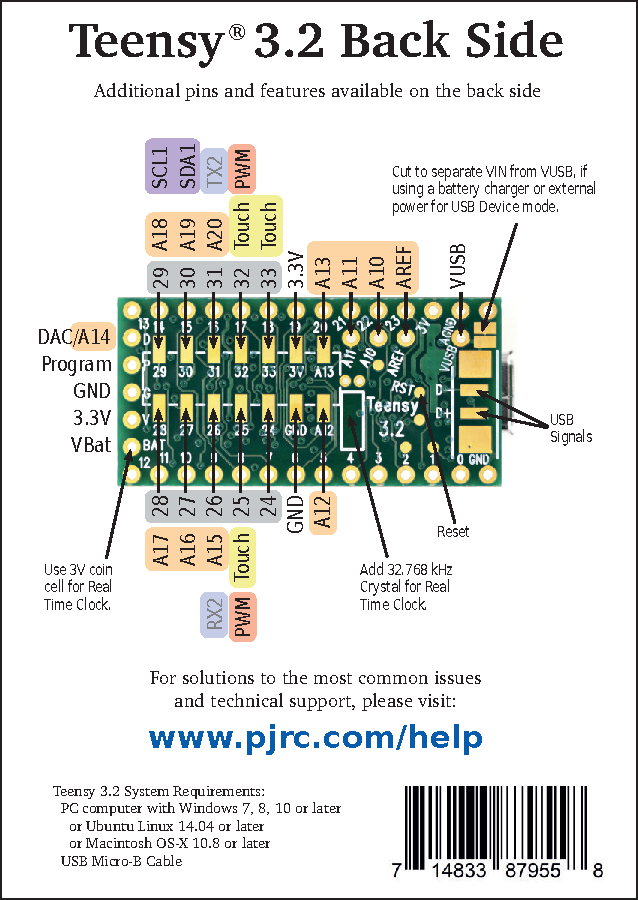
\includegraphics[width=6cm]{images/Teensy3.2 - 2.pdf}
    \caption{Pin map of Teensy 3.2}
    \label{Teensy3.2}
\end{figure}

It needs $3.2\mathrm{~V}$ of power supply and uses Teensyduino for coding, which is a software add-on for the Arduino to run sketches on the Teensy. The basic information is shown below (Table \ref{Specification of Teensy 3.2}). Overall, the Teensy board can communicate faster than other Arduino boards.

% it's one of the revised versions of \textit{Arduino} for use in \textit{Teensy3.2}. IDE is the same as \emph{Arduino}, but the compiler is different since \textit{Teensy} is not compatible with \textit{Uno, Nano}, and other Arduino boards. Here is the basic information:

% https://www.pjrc.com/teensy/teensyduino.html

 \begin{table}[H]
     \centering
     \begin{tabular}{l}
        \hline
        ARM Cortex-M4 at 72 MHz\\
        256K Flash, 64K RAM, 2K EEPROM\\
        \textbf{USB device 12 Mbit/sec}\\
        34 digital input/output pins, 12 PWM output pins\\
        21 analog input pins, 1 analog output pin, 12 capacitive sense pins\\
        3 serial, 1 SPI, 2 I2C ports\\
        1 I2S/TDM digital audio port\\
        1 CAN bus\\
        16 general purpose DMA channels\\
        RTC for date/time\\
        \hline
     \end{tabular}
     \caption{Specification of \textit{Teensy3.2}}
     \label{Specification of Teensy 3.2}
 \end{table}

DRV8825 and ST-M5045 are motor drivers which regulate step motors. DRV8825 was used for a small motor for testing out codes, and ST-M5045 was used to run a bigger motor, such as the one attached to a linear actuator. The specifications of the two motor drivers are shown below (Table \ref{Specification of DRV8825}, \ref{Specification of ST-M5045}).

\begin{figure}[H]
    \begin{center}
        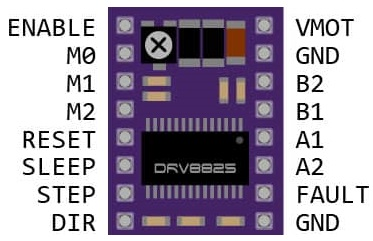
\includegraphics[height=4.5cm]{images/drv8825 pinmap.jpg}
        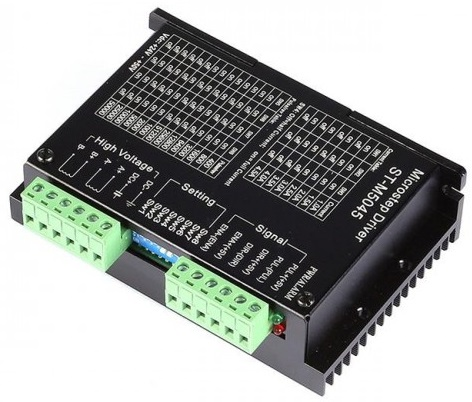
\includegraphics[height=4.5cm]{images/st-m5045.jpg}
    \end{center}
        \begin{tikzpicture} [remember picture, overlay]
        \node at (2.0, 0.5) {(a)};
        \node at (8.5, 0.5) {(b)}; %1.1
        \end{tikzpicture}	
        \caption{Motor drivers - (a) DRV8825 (b) ST-M5045}
        \label{Circuit - PCB, Schematic}
\end{figure}

\begin{table}[H]
    \centering
    \captionsetup{justification = centering}
    \begin{tabular}{ll}
        \hline
        % Number of full bridges           & 2                  \\
        Vs (min) $(\mathrm{V})$                     & 8.2                \\
        Vs ABS (max) $(\mathrm{V})$                 & 47                 \\
        Full-scale current $(\mathrm{A})$           & 2.5                \\
        Peak output current $(\mathrm{A})$          & 3                  \\
        RDS(ON) (HS + LS) $(\mathrm{m\Omega})$           & 400                \\
        Sleep current $(\mathrm{\mu A})$               & 10                 \\
        Control mode                     & STEP/DIR           \\
        Control interface                & Hardware (GPIO)    \\
        \textbf{Microstepping levels}             & \textbf{32}                 \\
        % Features                         & Current Regulation \\
        % Rating                           & Catalog            \\
        Operating temperature range $(\mathrm{\deg C})$ & -40 to 85         \\
        \hline
    \end{tabular}%
    \caption{Specification of \textit{DRV8825}}
    \label{Specification of DRV8825}
\end{table}

\begin{table}[H]
    \centering
    \captionsetup{justification=centering}
    \begin{tabular}{ll}
        \hline
        \textbf{DC power input type $(\mathrm{V})$}  & \textbf{24$\sim$50}      \\
        \textbf{Output current $(\mathrm{A})$}       & \textbf{1$\sim$4.5}      \\
        \textbf{Mircostep}           & \textbf{2, 4, 8, 16, 32, 64, 128, 256, 5, 10, 25, 50, 125, 250               }                \\
        Protect form        & Overheated, Short-voltage, over-voltage, over-current protection \\
        Maximum pulse rate $(\mathrm{kHz})$ & 300             \\
        Dimensions               & $120\mathrm{~mm}\times92\mathrm{~mm}\times33\mathrm{~mm}$ \\
        % Weight                   & \textless{}280g \\
        Working environment & Temperature-$15\sim40\mathrm{\deg C}$, Humidity\textless{}$90\%$ \\ 
        \hline
    \end{tabular}
    \caption{Specification of \textit{ST-M5045}}
    \label{Specification of ST-M5045}
\end{table}

Though DRV8825 is a small diode, it could function as well as other motor drivers, and it could be added to the PCB design so that the motor is controlled directly. But it tended to malfunction at high speeds and acceleration conditions. It's mainly due to the affordable voltage and current of the diode, and ST-M5045 was used for better control at higher voltage and current conditions. Also, the number of steps for each diode could be changed, which is related to the pulse is frequency. ST-M5045 is an exterior step motor driver and there are several switches at the side for changing the current and number of steps. To supply the whole system with proper power, a transformer is demanded. $24\mathrm{~V}$ SMPS converts AC voltage to DC $24\mathrm{V}$ and other versions can supply $36\mathrm{V}$ and $48\mathrm{V}$. With all these diodes, the final circuit was designed. (Figure \ref{Circuit - PCB, Schematic}).

\begin{figure}[H]
    \begin{center}
        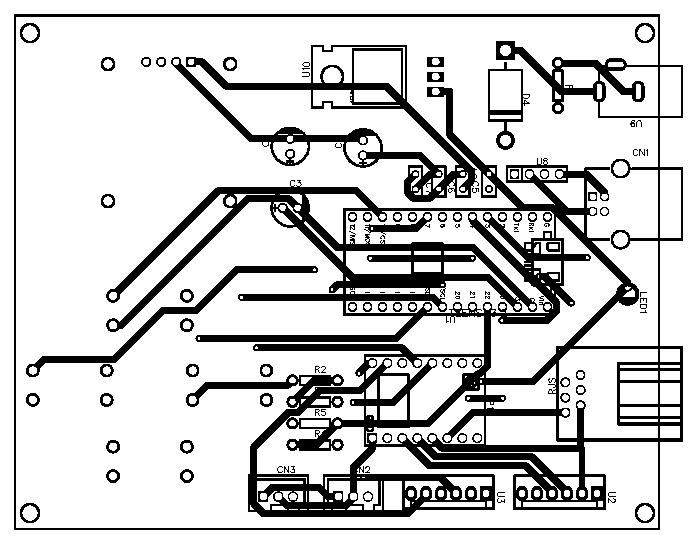
\includegraphics[width=9cm, angle=90]{images/Circuit(PCB).pdf}
        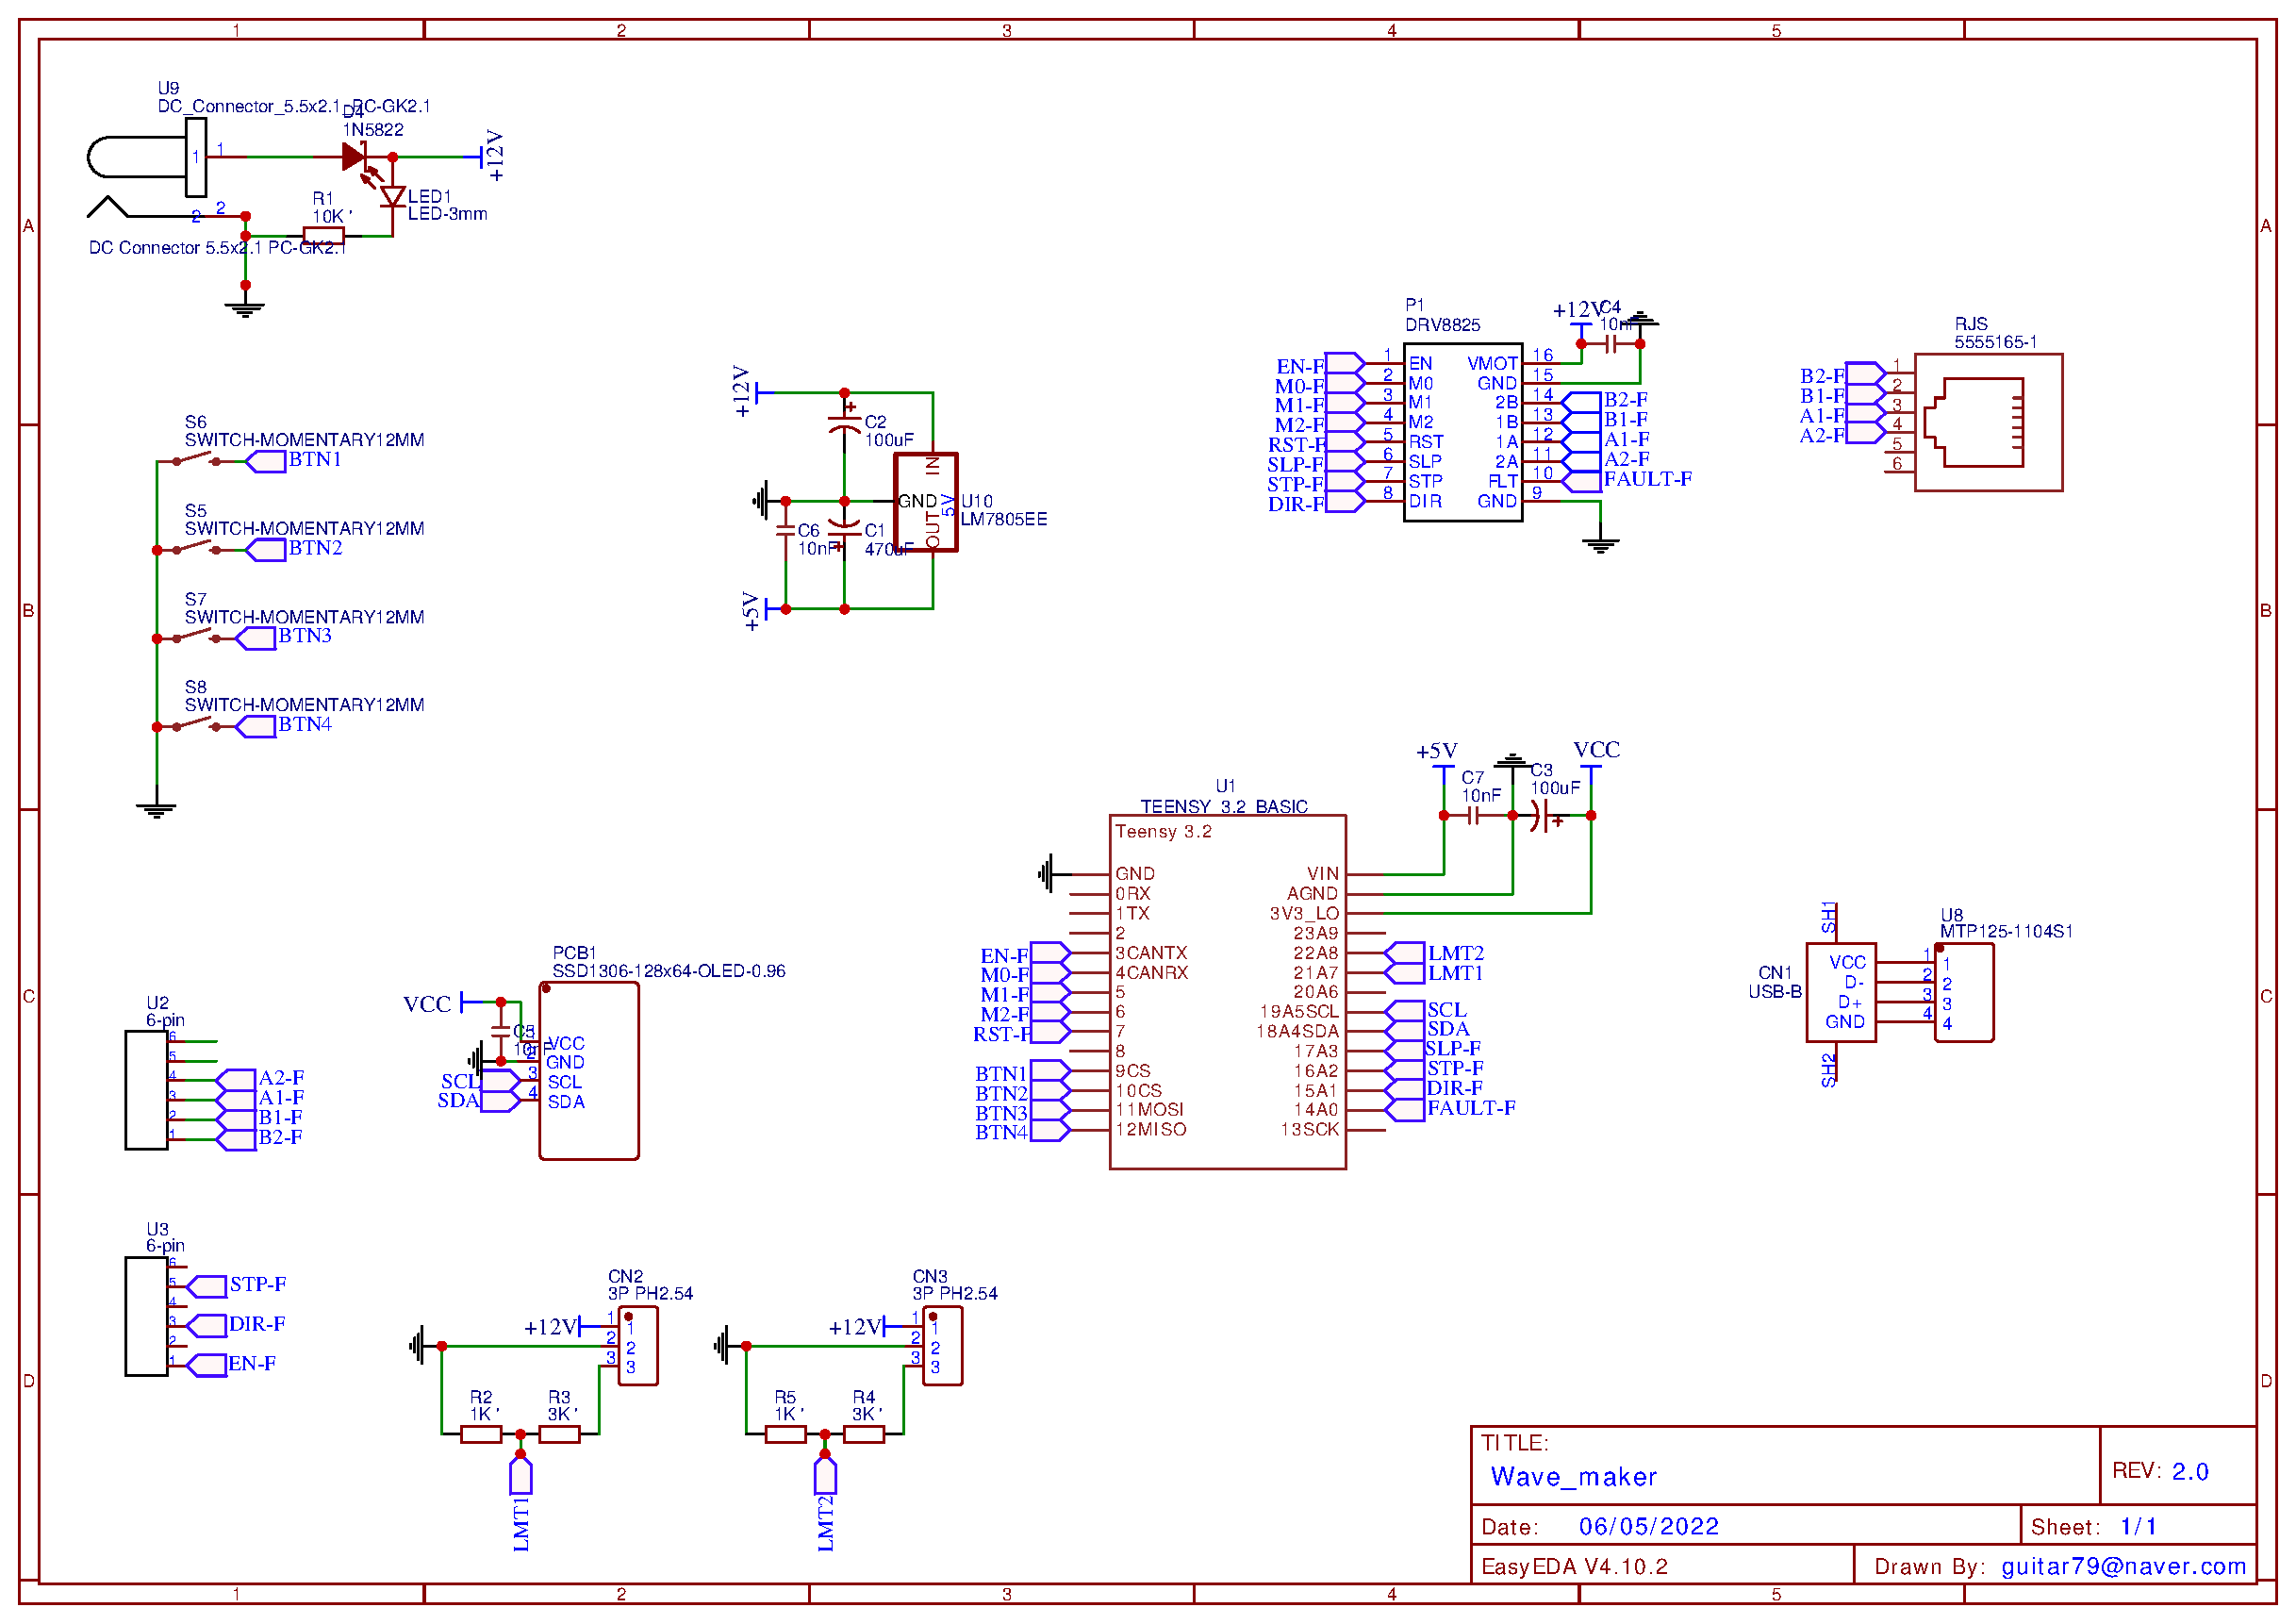
\includegraphics[width=9cm, angle=90]{images/Circuit(Schematic).pdf}
    \end{center}
        \begin{tikzpicture} [remember picture, overlay]
        \node at (0.9, 0.5) {(a)};
        \node at (7.9, 0.5) {(b)}; %1.1
        \end{tikzpicture}	
        \caption{Circuit - (a) PCB (b) Schematic diagram}
        \label{Circuit - PCB, Schematic}
\end{figure}

\subsubsection{Coding}
First of all, a fundamental code was made, which moves the plate back and forth. There are various libraries for driving a step motor and AccelStepper was used for it. Most of the libraries control the rotational speed of the motor. In the case of AccelStepper, it sets the angular velocity of the motor or the increment of the angular displacement, moving on a uniform velocity. 

\begin{algorithm}[H]
    \caption{Linear Movment}
    \label{Linear Movement}
    \begin{algorithmic}[1]
    \Statex Stepper motor(stepPin, dirPin);
    \Statex StepControl controller;
    \State \Comment{These variables and parameters should be defined priory}
    \Procedure{Linear Movement}{}\Comment{Move the motor back and forth}
        \Function {move motor}{$A$}
            \State motor.setTargetRel($A$);
            \State \Comment{moves the motor by $A$ steps}
            \State controller.move(motor);
            \State \Comment{$delay(time)$ is required!}
        \EndFunction
    \EndProcedure
    \end{algorithmic}
\end{algorithm}

The motor moved far slower than the expectation. Even though the maximum angular velocity and its angular displacement were set, the motor had limits according to the voltage, current, and performance of the motor driver. The transformer was changed so that higher voltage and current can flow through the circuit. It's raised to $36\mathrm{~V}$ from $24\mathrm{~V}$. Also, the code had changed. The new library is Teensystep \cite{luni64}. It can set the angular displacement of the motor as a function of time. By substituting the function from Algorithm \ref{Sinusoidal Motion}, a simple transverse motion and a sinusoidal move were able to be performed.

\begin{algorithm}[H]
    \caption{Time-based Motion}
    \label{Sinusoidal Motion}
    \begin{algorithmic}[1]
    \Procedure{Motion}{$A, \Delta t, \Delta\phi$}\Comment{Move the motor by setting angular displacement}
        \For{$elapsed Time \geq 0$}
            \If{$elapsed Time$ $\geq$ $\Delta t$}
                \State {$elapsed Time$ = 0}
                \State {$target = f(n)$}\Comment{For the sinusoidal motion, $target$ = $A \sin${($n$ $\Delta$$\phi$)}}
                % \State {$target$ = $A \sin${($n$ $\Delta$$\phi$)}}
                \State {$n$ $\gets$ $n$ + 1}
                \State {Move $motor$ to $target$}
            \EndIf
        \EndFor
        \EndProcedure
    \end{algorithmic}
\end{algorithm}

From Algorithm \ref{Sinusoidal Motion}, $f(n)$ is a function of dummy variable $n$, which sets $target$ - the angular displacement of the step motor - and $n$ is incremented by 1 in every $elapsedTime$. The code functions by setting the angular velocity of the motor based on $f(n)$, and there are other factors multiplied by it. $f(n) = A\sin{n \Delta\phi}$ is used to generate sinusoidal movement, with the proper value for the parameters. Here is an explanation of the parameters:
\begin{itemize}
    \item $A$

    It's the amplitude of the motion. Ideally, the plate should oscillate with the amplitude of $A$. It is measured in $step$, and it was known that 1$\mathrm{~cm}$ is equal to 400$\mathrm{~step}$, so the actual amplitude of the plate is $A/400$ in $\mathrm{~cm}$.

    \item $\Delta\phi$

    It's the increment of the phase of the displacement function with the dimension of $\mathrm{rad}$.

    \item $\Delta t$

    It's the value of $elapsedTime$ in the Algorithm \ref{Sinusoidal Motion}. Measured in $\mathrm{ms}$ with $millis()$, it sets the time interval for increasing dummy variable $n$.
\end{itemize}

The phase velocity(the rate at which phase of the function $f(n)$ changes) is derived as:
\begin{equation}
    \omega = \frac{\Delta\phi}{\Delta t}
    \label{Code: Omega}
\end{equation}

By setting $A$, $N(=\Delta t)$ and $\omega$ as a new parameter, $\Delta \phi$ is deleted and $f(n)$ as a function of $\omega$ is derived:
\begin{equation}
    f(n) = A\sin{N\omega}
    \label{Code: New f(n) with parameter omega}
\end{equation}

The whole process of the wavemaker is shown in Figure \ref{Flow chart of the wave generating system}. As the parameters were set, the plate was moved by the code, and the wave was generated.

\begin{figure}[H]
    \centering
    \captionsetup{justification=centering}
    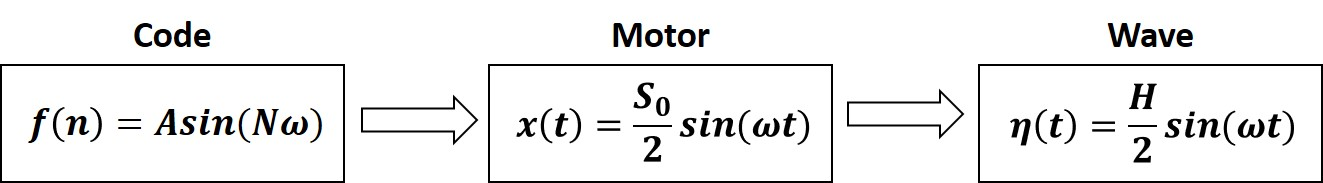
\includegraphics[width=12cm]{images/Flow_Chart(Analysis System).jpg}
    \caption{Flow chart of the wave generating system}
    \label{Flow chart of the wave generating system}
\end{figure}

All three sinusoidal functions share the same phase velocity $\omega$, and amplitudes have certain relations in between(Refer to Equation \ref{eq_023} and description of the parameters).

\subsection{Wave Gauge}%Check!

% \begin{figure}[H]
%     \begin{center}
%         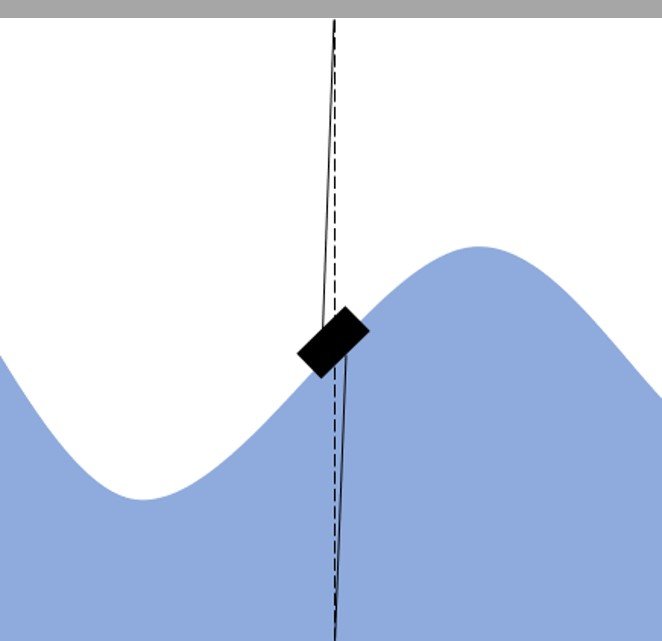
\includegraphics[height=6cm]{images/Wave_Gauge(Illustrated).jpg}
%         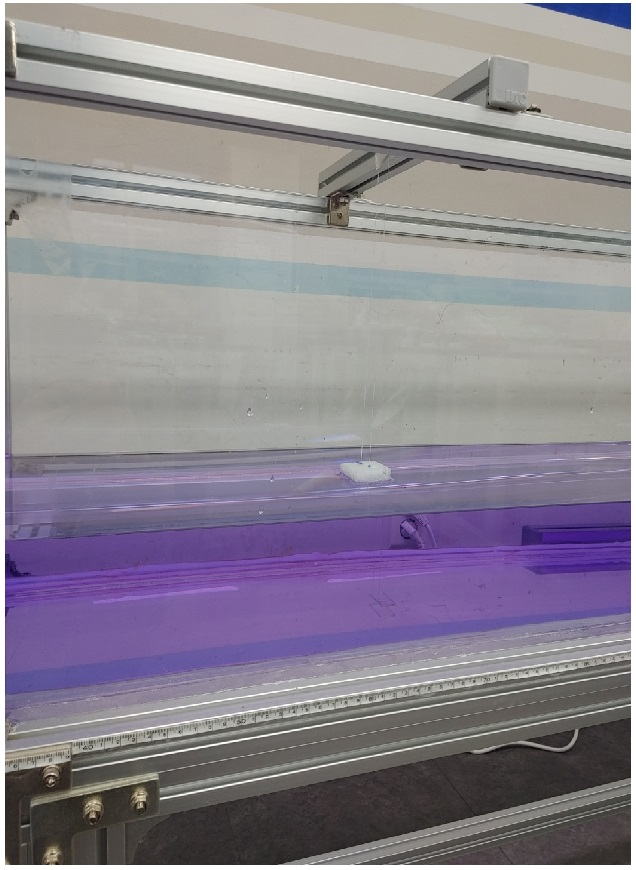
\includegraphics[height=6cm]{images/Wave_Gauge.jpg}
%     \end{center}
%         \begin{tikzpicture} [remember picture, overlay]
%         \node at (2.0, 0.5) {(a)};
%         \node at (7.0, 0.5) {(b)}; %1.1
%         \end{tikzpicture}	
%         \caption{Wave gauge - (a) Illustration (b) }
%         \label{Wave gauge}
% \end{figure}

\begin{figure}[H]
    \centering
    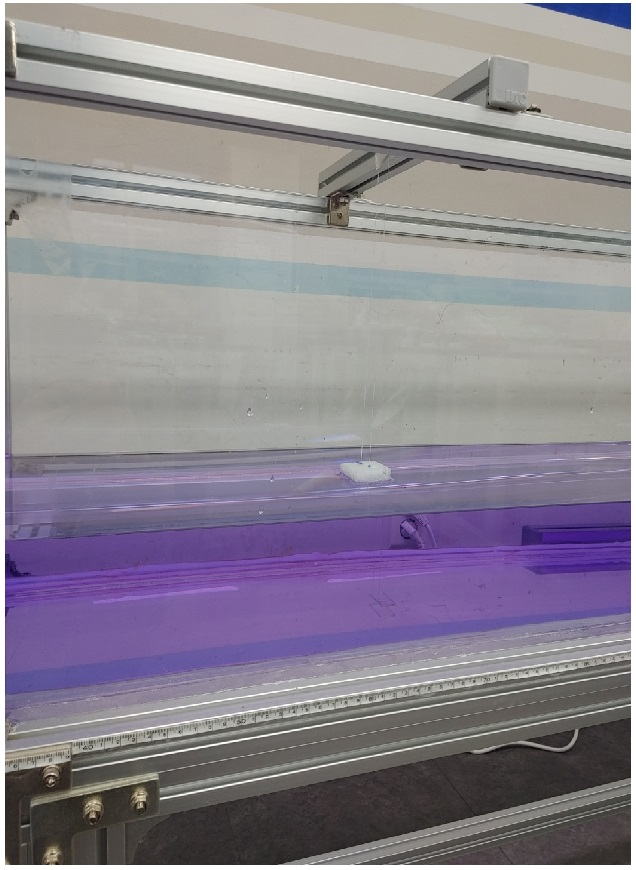
\includegraphics[height=8cm]{images/Wave_Gauge.jpg}
    \caption{Wave gauge}
    \label{Wave gauge}
\end{figure}

Wave height data was needed to derive the phase velocity and amplitude of the wave. A buoy was put on the water to measure the wave height and its movement was recorded. The buoy was fixed horizontally so that only the vertical movement was tracked properly. The size of the buoy was small so it don't affect the wave. A piece of Styrofoam was used, and it was fixed to the bottom and an assistant metal bar at the top of the wave channel with a thin string (Figure \ref{Wave gauge}). A dot was drew on one side of the buoy for video analysis, but it kept rotating by the external impulse. So, two strings were used to stop the rotation.
%Bookmark
Also, the water was pigmented blue to increase the contrast between the water and the buoy. It gives a better condition for the Tracker program, a video tracking \& analyzing tool.

\subsection{Code Test}
\begin{align*}
    Code: f(n) &= A \sin{N \omega_{1}}\\
    Motor: x(t) &= S_{0} \sin{\omega_{2} t}\\
    Wave: \eta(t) &= H \sin{\omega_{3} t}
\end{align*}

Out of the three sinusoidal waves shown above, the following is assumed:
\begin{align*}
    Amplitude&: A = S_0, H = \frac{4 S_0 \sinh^2 {kh}}{\sinh{2kh} + 2kh}\\
    Frequency&: \omega_{1} = \omega_{2} = \omega_{3}
\end{align*}

From testing out the code with the small motor and comparing $f(n)$ and $x(t)$, the phase velocity had agreed, but the amplitude was different (Figure \ref{PreExperiment}).

\begin{figure}[H]
    \centering
    \begin{tabular}{ll}
        \begin{filecontents*}{A.dat}
w_msr	A_thm	A_msr
0.6272	10	9.515
0.6275	10	9.532
0.6541	10	9.523
0.6681	10	9.499
0.6826	10	9.48
0.6978	10	9.456
0.6978	10	9.449
0.7849	10	9.326
0.785	10	9.318
0.8263	10	9.26
0.8971	10	9.138
0.8971	10	9.137
1.047	10	8.883
1.047	10	8.876
1.256	10	8.498
1.256	10	8.492
1.57	10	7.916
1.57	10	7.903
1.744	10	7.588
1.962	10	7.206
1.962	10	7.197
2.093	10	6.988
2.093	10	6.978
2.243	10	6.749
2.415	10	6.489
2.617	10	6.218
2.618   10	6.214
3.141	10	4.837
3.141	10	4.837
3.927	10	3.093
5.236	10	0.5795
        \end{filecontents*}

        \begin{tikzpicture}[
                %Environment Cfg.
                %font=\bfseries\sffamily,
            ]
            \begin{axis}[
                width=7cm,
                height=7cm,
                at={(0,0)},
                ymin=0,
                ymax=13,
                xmin=0,
                xmax=6,
                grid=both,
                minor tick num =5,
                minor tick style={draw=none},
                minor grid style={thin,color=black!10},
                major grid style={thin,color=black!10},
                %ylabel style={rotate=90},
                ylabel={$A_{plate}~\left[\mathrm{~cm}\right]$},
                xlabel={$\omega_{msr}~\left[\mathrm{~rad/s}\right]$},
                tick align=outside,
                axis x line*=middle,
                axis y line*=none,
                xtick={0,2,...,16},
                ytick={0,2,...,16},
                %xlabel style={color=blue!50!cyan},
                %ylabel style={align=center,rotate=-90,color=blue!50!cyan},
                x tick label style={
                    /pgf/number format/assume math mode, font=\sf\scriptsize},
                y tick label style={
                    /pgf/number format/assume math mode, font=\sf\scriptsize},
                legend cell align = {left},
                legend pos = north west,
                legend style={nodes={scale=0.5, transform shape}},
                ]
                \addplot [%only marks, 
                    mark size=1pt,
                    mark=o, 
                    %mark options={solid}, 
                    %smooth,
                    ] 
                table [x=w_msr, y=A_thm] {A.dat};
                \addlegendentry{$A_{thm} - \omega_{msr}$}
                \addplot [%only marks, 
                    mark = +,
                    mark size=1pt,
                    ]
                table [x=w_msr, y=A_msr] {A.dat};
                \addlegendentry{$A_{msr} - \omega_{msr}$}
            \end{axis}
        \end{tikzpicture}
        
        &
        
        \begin{filecontents}{B.dat}
                    wthm   wPlate
0.6283	0.6272
0.6981	0.6978
0.7854	0.785
0.8976	0.8971
1.0472	1.047
1.2566	1.256
1.5708	1.57
1.9635	1.962
2.0944	2.093
2.6180	2.617
3.1416	3.141
3.9270	3.918
5.2360	5.236
4.4880	4.487
3.9270	3.919
3.4907	3.49
0.6283	0.6275
0.6545	0.6541
0.6684	0.6681
0.6830	0.6826
0.6981	0.6978
0.7854	0.7849
0.8267	0.8263
0.8976	0.8971
1.0472	1.047
1.2566	1.256
1.5708	1.57
1.7453	1.744
1.9635	1.962
2.0944	2.093
2.2440	2.243
2.4166	2.415
2.6180	2.617
3.1416	3.141
            \end{filecontents}
        
            \begin{tikzpicture}[
                    %Environment Cfg.
                    font=\bfseries\sffamily,
                ]
                    \begin{axis}[
                        width=7cm,
                        height=7cm,
                        at={(0,0)},
                        ymin=0,
                        ymax=6,
                        xmin=0,
                        xmax=6,
                        grid=both,
                        minor tick num =5,
                        minor tick style={draw=none},
                        minor grid style={thin,color=black!10},
                        major grid style={thin,color=black!10},
                        %ylabel style={rotate=90},
                        ylabel={$\omega_{msr}~\left[\mathrm{rad/s}\right]$},
                        xlabel={$\omega_{thm}~\left[\mathrm{rad/s}\right]$},
                        tick align=outside,
                        axis x line*=middle,
                        axis y line*=none,
                        xtick={0,2,...,16},
                        ytick={0,2,...,16},
                        %xlabel style={color=blue!50!cyan},
                        %ylabel style={align=center,rotate=-90,color=blue!50!cyan},
                        x tick label style={
                            /pgf/number format/assume math mode, font=\sf\scriptsize},
                        y tick label style={
                        /pgf/number format/assume math mode, font=\sf\scriptsize},
                        legend cell align = {left},
                        legend pos = north west,
                        legend style={nodes={scale=0.5, transform shape}},
                        ]
                        \addplot [only marks, 
                            mark size=1pt,
                            mark=o, 
                            ]
                            table [x=wthm, y=wPlate] {B.dat};
                           \addlegendentry{$ \omega_{msr} - \omega_{thm}$}
                    \end{axis}
        \end{tikzpicture}
    \end{tabular}
    
    \begin{tikzpicture} [remember picture, overlay]
        \node at (-5.8, 0.6) {\scriptsize{(a)}};
        \node at (2.0, 0.6) {\scriptsize{(b)}};
    \end{tikzpicture}
    \caption{$\omega_{msr} - \omega_{thm}$ graph - (a) wave (b) plate}
    \label{PreExperiment}
\end{figure}

% \begin{figure}[H]
%     \centering
%     \captionsetup{justification=centering}
%     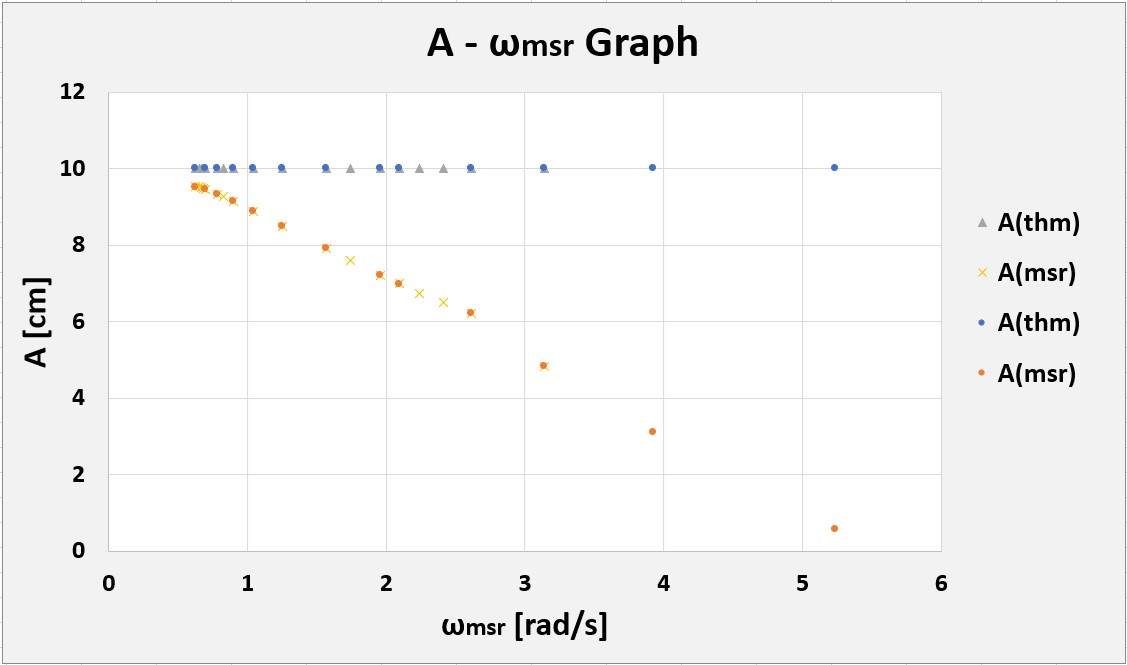
\includegraphics[width=12cm]{images/PreExperiment_Graph(A-Omega).jpg}
%     \caption{$A - \omega_{msr}$ Graph of motor}
%     \label{PreExperiment Graph(A - Omega)}
% \end{figure}

Angular displacement data had been collected from the Serial monitor and transitional data of the plate had been collected by tracking its movement from the video. $\omega$ was varied by changing $\Delta\phi$ and $N$. $A$ was fixed to $10\mathrm{cm}$ and it's expected to be consistent for the plate's motion. But instead, the measured amplitude had been smaller, and it seemed to decrease as $\omega$ increased. From Figure \ref{Circuit - PCB, Schematic}, orange dots were collected by changing $N$, and yellow dots were collected by changing $\Delta\phi$ (However, $\omega_{msr}$ refers to the measured value and $\omega_{thm}$ refers to the theoretically predicted value. $_{msr}$ and $_{thm}$ notation is used throughout the whole paper).

Unlike amplitude, $\omega_{msr}$ (measured $\omega$) agreed with $\omega_{thm}$ ($\omega$ in the code) with high precision. (Figure \ref{PreExperiment Graph(Omega - Omega)}). The best-fit line was $y=0.999510x$ with $R^2 = 1.000000$.

% \begin{figure}[H]
%     \centering
%     %\captionsetup{justification=centering}
%     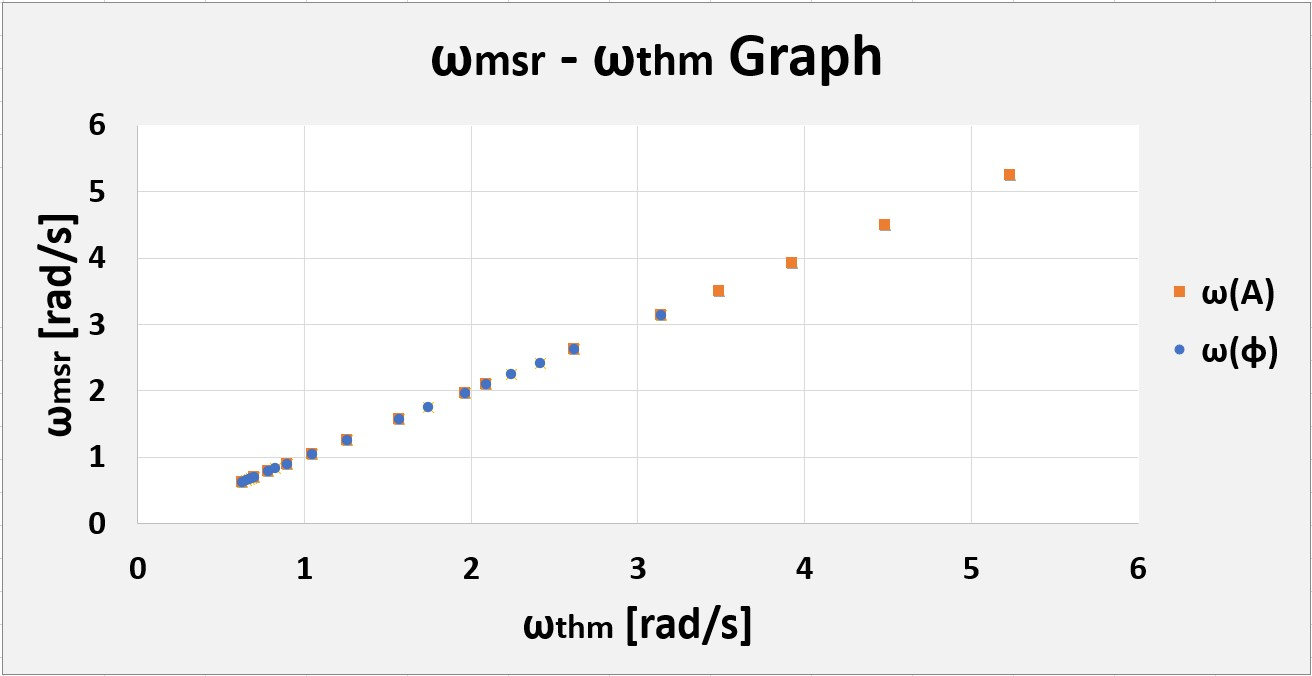
\includegraphics[width=12cm]{images/PreExperiment_Graph(Omega-Omega).jpg}
%     \caption{$\omega_{msr} - \omega_{thm}$ Graph of motor}
%     \label{PreExperiment Graph(Omega - Omega)}
% \end{figure}




It's concluded that this phenomenon was due to the limitation of the motor, related to parameters MaxSpeed and MaxAcceleration. The amplitude could be increased but the difference was inevitable. As $\omega$ increased, the plate couldn't catch up with the expected motion speed and acceleration. The reason is that the motor worked by calculating the velocity difference between the current and next states, and moved to the target though it hadn't reached the expected velocity. It resulted in a smaller amplitude and the wave got distorted. MaxSpeed and MaxAcceleration were set from the code but they're just numbers, and to increase the performance of the motor, provided voltage and current were raised. This problem was approached from a basic power supply issue.

Since $A$ and $S_{0}$ were different, three waves needed to be compared: signal from the code (angular displacement of the step motor), movement of the plate (transitional displacement), and progressive wave from in the channel(Figure \ref{Flow chart of the wave generating system}). There was no information of a relation between $A$ and $S_{0}$. The trend doesn't fit in $y=1/x$ (MaxSpeed = (const)) or $y=1/x^{2}$ (MaxAcceleration = (const)), and there were no other distinct trends related. But it's still assumed that the relation between $S_{0}$ and $H$ holds, and the relation between $A$ and $S_{0}$ will be collected for interpolation.

\subsection{Experimental Setup}
From the Code Test and Froude Similarity Law, various conditions for the experiments were set as $A~=~1,~2,~...,~10\mathrm{~cm}$ and $\omega~=~0.5\pi,~\pi,~...,~4.0\pi$. But, there had been some unexpected issues, and $\omega$ had changed to $3,~4,~6,~7,~9,~10,$ and $12\mathrm{~rad/s}$.


\begin{figure}[H]
    \begin{center}
        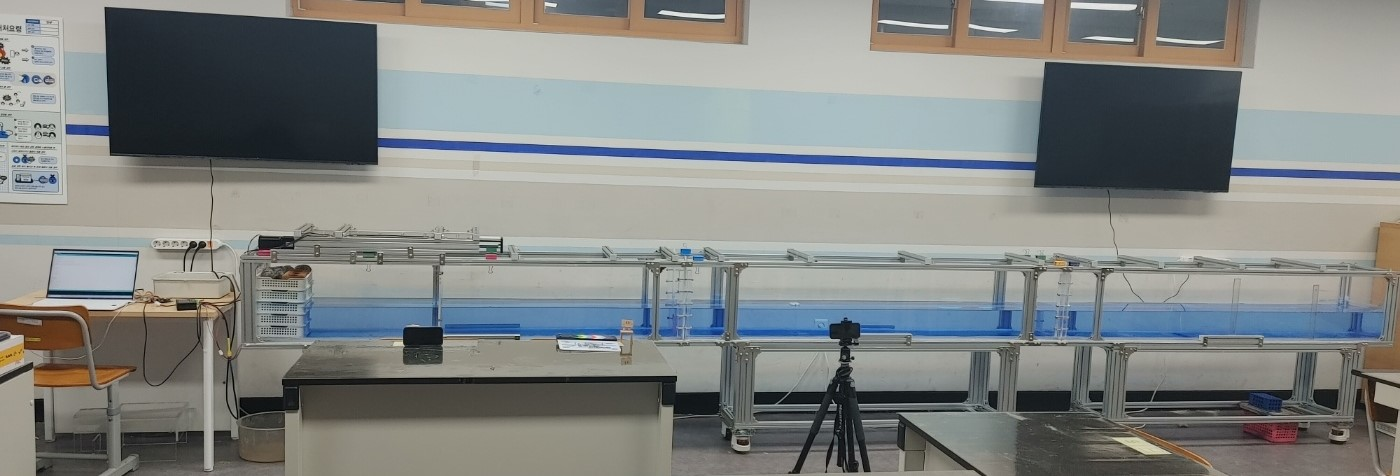
\includegraphics[width=\textwidth]{Experiment_System_Crop}
    \end{center}
        \begin{tikzpicture} [remember picture, overlay]
        \node [draw=yellow, text=yellow] (computer) at (1.0, 3.8) {\scriptsize{computer}};
        % \node [draw] (computer) at (1.0, 3.5) {.};
        % % arrows
        % \draw [->] (computer) -- (computerA) 
        \node [draw=yellow, text=yellow] at (4.6, 1.7) {\scriptsize{camera1}};
        \node [draw=yellow, text=yellow] at (9.5, 1.5) {\scriptsize{camera2}}; 
        \end{tikzpicture}	
        \caption{Experiment system - Laboratory}
        \label{Experimnet_System} 
\end{figure}


The system is shown in Figure \ref{Experimnet_System}. At the left end of the channel, the wave was generated, and there were two cameras beside the wave channel to collect data from the movement of the plate and the buoy.